\documentclass[../../main.tex]{subfiles}
\begin{document}

%A graph is considered \textit{directed} if it is represented by an ordered pair
%$G=(V,E)$, where $V$ is the set of vertices and $E$ is the set of directed
%edges or arcs. Conversely, undirected graphs are described by unordered pairs
%of vertices.
%
%Early efforts to define quantum walks on directed graphs were made by
%establishing conditions such as \textit{strong quadrangularity}
%\cite{severiniUnderlying03,severiniDigraph03} and \textit{graph reversibility}
%\cite{severiniUnderlying03,severiniDigraph03,montanaroQuantum05} as
%prerequisites for defining \textit{coined quantum walks} on directed graphs.
%More recent works demonstrate performance gains of the CTQW in the context
%of centrality ranking \cite{Caruso2016}, leading to applications to the
%PageRank algorithm \cite{Wang2020}. Other models were also defined in these
%structures, such as the \textit{staggered quantum walk} in oriented graphs
%\cite{chagas20}
%
%Directed graphs exhibit distinct transport properties compared to undirected
%graphs, thus requiring different methods to characterize state transfer
%\cite{godsilPerfect2020}. Additionally, these graphs can exhibit new phenomena, such
%as zero transfer \cite{Sett2019}, and certain initial conditions can result in
%dynamics that remain unchanged despite the addition of direction
%\cite{chaves2022}.
%
%In the following subsections, we will see how to use \texttt{QWAK} to produce
%the dynamics of a CTQW in a directed infinite line, as well as a demonstration
%of how to reproduce \textit{enhanced decay rate} \cite{abalEffects06} of the
%survival probability for more general structures. 


A directed graph $G=(V,E)$ differs from its undirected counterpart by having
ordered vertex pairs in $E$. Early work established \textit{strong
quadrangularity} and \textit{graph reversibility} as prerequisites for coined
quantum walks (CQWs) on such graphs
\cite{severiniUnderlying03,severiniDigraph03,montanaroQuantum05}. Recent
studies show performance gains in centrality ranking via CTQWs
\cite{Caruso2016}, with applications like PageRank \cite{Wang2020}. Other
models, like \textit{staggered quantum walks}, have also been defined
\cite{chagas20} in these structures.

Directed graphs exhibit distinct transport properties, requiring different
methods to characterize state transfer \cite{godsilPerfect2020}. Additionally,
these graphs can exhibit new phenomena, such as zero state transfer \cite{Sett2019}.
%and invariant dynamics under certain initial conditions \cite{chavesWhy22}.
%\textcolor{blue}{Esta parte do invariant dynamics corresponde a citacao do why
%and how?}

In the subsequent sections, we will demonstrate how to use \texttt{QWAK} for
simulating CTQWs on directed infinite lines and explore the \textit{enhanced
decay rate} of the survival probability \cite{abalEffects06} in more general
structures \cite{Chaves2023}.

\subsubsection{Dynamics}

To define a directed infinite line, as shown in figure \ref{fig:oriented_line},
we use the Hamiltonian $H$ given by equation 

\begin{equation}\label{hamiltonian}
    H = \sum_{x = L}^{R}e^{i\alpha}\ketbra{x+1}{x}+e^{-i\alpha}\ketbra{x-1}{x},
\end{equation}
where $L$ and $R$ are the left and right borders of
the line, respectively. We can obtain an infinite path graph by setting
$R\rightarrow\infty$ and $L\rightarrow -\infty$. 

\begin{figure}[!h]
    \centering
    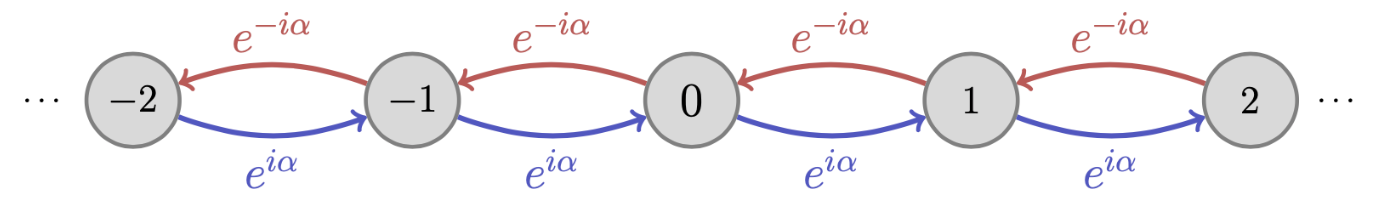
\includegraphics[width=12cm]{img/QWAK/oriented_infinite_line.png}
    \caption{Directed infinite line with weights $e^{i\alpha}$ and $e^{-i\alpha}$.}
    \label{fig:oriented_line}
\end{figure}

We implement the \textit{finite} line using the \texttt{path\textunderscore
graph} function and add direction to it using the \texttt{getWeightedGraph}
function available in the notebook.

\begin{lstlisting}[style=code,escapeinside={__}]
n = 100
alpha = np.pi/2
weight = np.exp(1j*alpha)
baseGraph = nx.path_\textunderscore_graph(n,create_\textunderscore_using=nx.DiGraph)
graph = getWeightedGraph(baseGraph,weight)
\end{lstlisting}

Inspired by previous work \cite{abalEffects06}, we choose a non-localized
initial condition given by equation

\begin{equation}
    \label{eq:survProbInitCond}
    \ket{\psi(0)} = \cos(\theta)\ket{-k} + e^{i\gamma}\sin(\theta)\ket{k},
\end{equation}


which can be easily implemented in Python. 

\begin{lstlisting}[style=code,escapeinside={__}]
k = 1
theta=np.pi/4
l = 0
gamma = l * np.pi

initCond = [(n//2-k,np.cos(theta)),(n//2+k,np.exp(1j*gamma)*np.sin(theta))]
\end{lstlisting}

Once all the necessary components are in place, generating the distribution for
this example follows a similar procedure to that outlined in Section
\ref{sec:OverviewDescription}. After initializing the \texttt{QWAK} object, we
compute the  walk using the \texttt{runWalk} method. To specify a
non-localized initial condition, we pass the \texttt{customStateList} parameter
to provide both the node and its corresponding amplitude.

\begin{lstlisting}[style=code,escapeinside={__}]
t = 35

qw = QWAK(graph)
qw.runWalk(time = t,customStateList = initCond)

probVec = qw.getProbVec()
\end{lstlisting}

The probability distribution is obtained using the \texttt{getProbVec} method. To
study how the evolution of the probability distribution changes with different
graph weights, Fig. \ref{fig:multipleAlphaOrientedDynamics} displays the CTQW
for multiple values of $\alpha$.

\begin{figure}[!h]
    \centering
    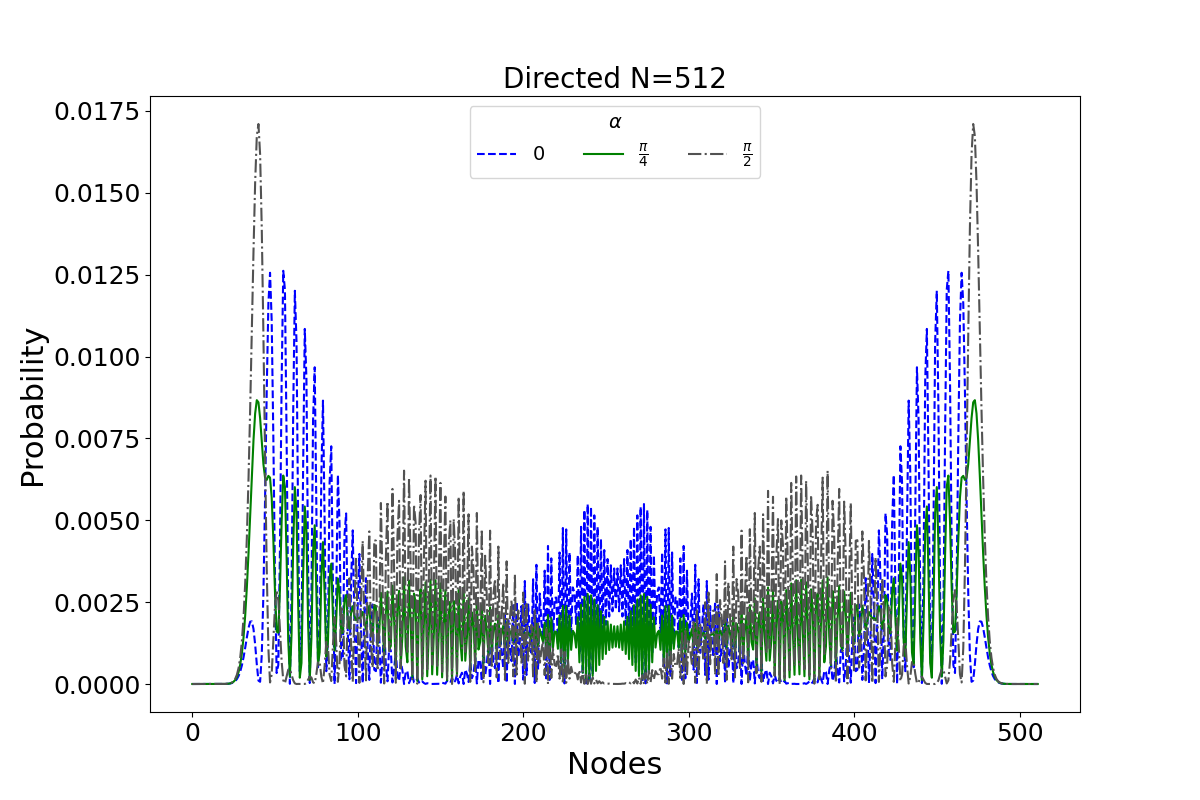
\includegraphics[scale=\mysinglefigurescale]{img/QWAK/OrientedDynamics/orDynN512NW3Alpha0.79-1.57TMAX110.png}
    \caption{Probability distribution for the CTQW on a 
        directed finite line of size $N=512$, at $t=110$, with initial condition  $\ket{\psi(0)}=\frac{\ket{253}+\ket{259}}{\sqrt{2}}$
    and $\alpha = 0$, $\frac{\pi}{4}$ and $\frac{\pi}{2}$.}
    \label{fig:multipleAlphaOrientedDynamics}
\end{figure}

Indeed, the value of $\alpha$ has a severe impact in the dynamics of the walk.
In the case of an undirected graph ($\alpha = 0$), symmetry is expected around
the center node; however, varying values of $\alpha$ can alter the shape of the
distribution, presenting a method of controlling how the walker propagates
throughout the structure.

\subsubsection{Survival Probability}
The survival probability of a quantum walk can be characterized as the mean
probability of finding the walker in a certain location after some time $t$
\cite{Goenuelol2011}. Considering the symmetric position range of $[k_0,k_1]$, this
quantity will be
\begin{equation}
    P_{[k_0,k_1]}(t)=\sum_{i=k_0}^{k_1} P_{i}(t).
\end{equation}

Here, we will use \texttt{QWAK} to run the walk for a interval using multiple
values of $\alpha$. Classically, the survival probability decays at a rate
proportionate to $t^{-\frac{1}{2}}$, while a quantum walk typically decays
quadratically faster at a rate of $t^{-1}$. It is known, however, that certain
initial conditions can achieve \textit{enhanced decay rate}
\cite{abalEffects06}, scaling with $t^{-3}$.\par

\begin{figure}[!h]
    \centering
    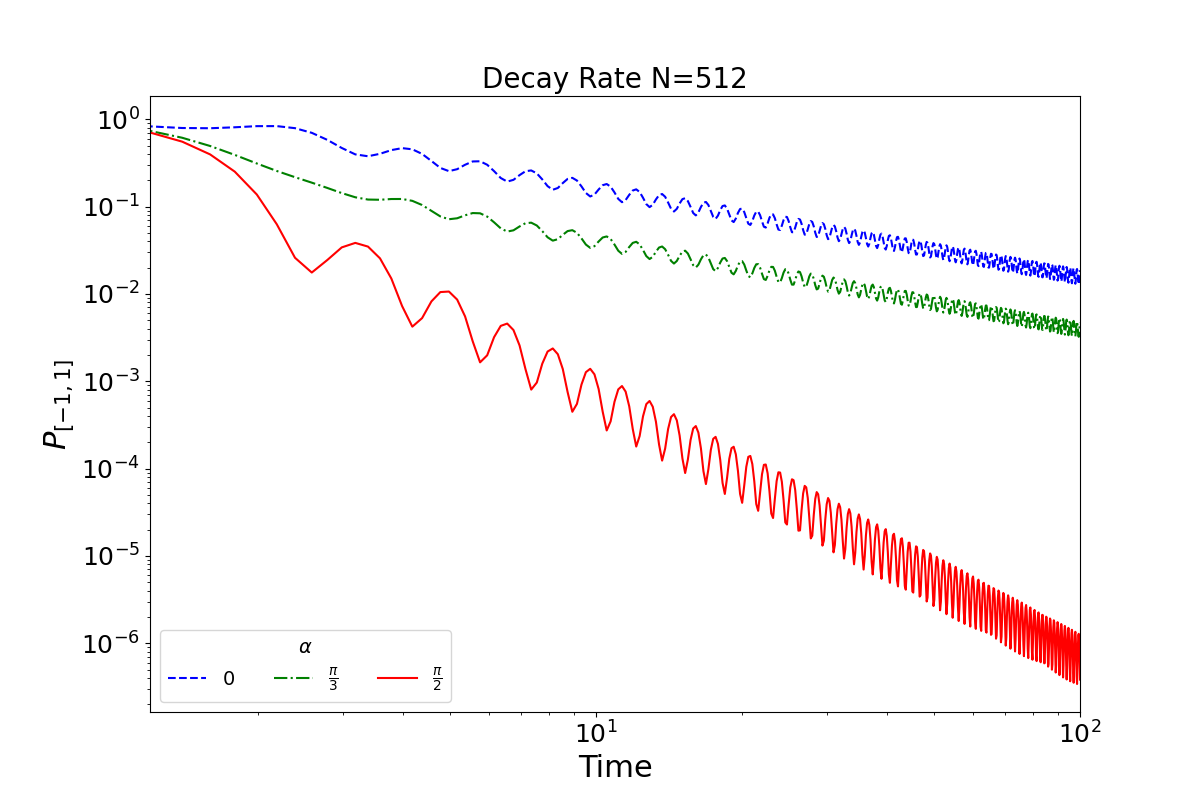
\includegraphics[scale=\mysinglefigurescale]{img/QWAK/OrientedDecayRate/decMatrix512NW3_Alpha1.05-1.57S500TMAX100.png}
    \caption{Decay of the survival probability on a directed infinite line of
        size $N=512$, for $\theta =\frac{\pi}{4}$, $\gamma=0$, and $\alpha=0$,
        $\frac{\pi}{2}$ and $\frac{\pi}{3}$.}
    \label{fig:decay_rate_oriented_line}
\end{figure}

Using the previously defined directed graph and the chosen initial condition, we
can analyze the impact of varying $\alpha$ values on the decay rate of the
survival probability:

\begin{lstlisting}[style=code]
timeList = np.linspace(0,100,500)
alphaList = [0, np.pi/3, np.pi/2]
decayRateMatrix = []
for alpha in alphaList:
    weight = np.exp(1j * alpha)
    graph = getWeightedGraph(baseGraph, weight)
    qw = QWAK(graph)
    qw.runMultipleWalks(timeList, customStateList=initCond)
    decayRateMatrix.append(
                  qw.getSurvivalProbList(N//2 - k, N//2 + k))

plt.loglog()
for decayRate in decayRateMatrix:
    plt.plot(survProbList)
plt.show()
\end{lstlisting}

The code iterates through a list of $\alpha$ values, generating a directed
graph for each and computing the corresponding survival probabilities over
time. These are stored in a decay rate matrix for log-log plotting, as shown in
Fig. \ref{fig:decay_rate_oriented_line}.

As demonstrated in Chaves et al \cite{Chaves2023}, directional line graphs
enable more effective control of interference effects in quantum walks. This
allows for both normal and enhanced decay rates under broader initial
conditions. The figure shows that an optimal $\alpha$ value can be chosen to
accelerate decay, irrespective of $k$'s parity.

\end{document}
